\documentclass[../main.tex]{subfiles}

\begin{document}

El corazón humano contrae sus músculos mediante pulsos eléctricos, pero en algunos casos estos no son capaces de ser generados regularmente. El continuo progreso de la ciencia ha permitido la creación de dispositivos llamados marcapasos cada vez más avanzados cuya función es generar estos pulsos y así mejorar la salud del corazón del paciente. Los impulsos eléctricos son creados mediante los llamados \textit{circuitos de estímulos}, que no es más que un conjunto de resistencias y condensadores unidos a una fuente de alimentación; o lo que es lo mismo, un circuito RC. \cite{intro_circuitos_RC} \\

Las aplicaciones de este tipo de circuitos no se centran solamente en el área de la medicina, sino que también podemos encontrarlos en objetos de uso cotidiano. Si observamos algunos de los auriculares de última generación que llevan incorporados una serie de funciones que permiten aislar ruido del exterior, vemos que estos utilizan lo que se conoce como \textit{filtros de paso}, que dependiendo de si se quieren escuchar frecuencias altas, bajas o en un rango, se utilizarán respectivamente los filtros de paso alto, bajo o de banda. Estos filtros no son más que circuitos RC dónde sus componentes se encuentran dispuestos de diferente manera según el objetivo que se quiere conseguir. Y, aunque normalmente las frecuencias de filtrado ya vienen configuradas de fábrica, existen modelos en los que estas pueden cambiarse mediante el uso de resistencias variables.\\

Otro uso de estos circuitos serían en las \textit{fuentes de luz estroboscópicas}. Se trata de una fuente de luz cuya emisión se produce de forma intermitente. Este tipo de dispositivos podemos encontrarlos en los \textit{strobes} de un avión (los focos de color rojo y verde que se sitúan en los extremos de las alas y cuya función es posicionar a la aeronave para evitar colisiones) o en cámaras de fotografía para tomar instantáneas de objetos en movimiento, como se puede ver en la figura \ref{foto_estroboscópica}.\\

\begin{figure}[!h]
          \centering
          \includegraphics[width=0.5\textwidth]{images/foto_estroboscópica.png}
          \caption{Movimiento de un balón usando una \textit{cámara estroboscópica}.}
          \label{foto_estroboscópica}
\end{figure}

Por otro lado tenemos los circuitos RL. Un ejemplo de uso de este tipo de circuitos lo encontramos durante el proceso de combustión en un motor de gasolina. Para que esta se lleve a cabo, el combustible debe de mezclarse con una serie de gases inflamables a alta presión y posteriormente, se debe de producir una chispa que queme esta mezcla. Para ello se hace uso de las bujías, unos dispositivos compuestos por dos hilos separados entre sí entre los que se produce una alta diferencia de potencial creando así un arco voltaico que es capaz de iniciar la combustión en el interior del motor. Pero normalmente los vehículos que emplean estos motores suelen ser alimentados por baterías de 12V o 24V, siendo estos voltajes insuficientes para que las bujías puedan llegar a inducir esa chispa.\\

Además de en motores de combustión de gasolina, este tipo de circuitos podemos hallarlos en dispositivos de filtrado de frecuencia (similares a los construidos con circuitos RC) o en circuitos osciladores. Estos últimos pueden usarse para la construcción de generadores de ondas de radio o televisón y en receptores usados en la telefonía móvil. Estos se encuentran formados por una serie de condensadores, resistencias y bobinas conectadas, también llamados circuitos RLC. Aunque estos sean otro caso de uso de bobinas y condensadores, estos circuitos no son objeto de estudio en este trabajo así que a continuación, nos centraremos en el estudio de los circuitos RC y RL en corriente continua y estado transitorio.


\subsection{El condensador y el circuito RC}
En primer lugar, comenzamos definiendo qué es un condensador. Este se trata de un dispositivo compuesto generalmente por dos placas conductoras aisladas entre sí, a través de un medio vacío, aire o algún material aislante; comunmente llamado diélectrico, en el que podemos almacenar energía eléctrica.\\ 

La cantidad de energía que puede almacenarse en un condensador depende de la relación que existe entre la carga de cada una de las armaduras y de la diferencia de potencial que se aplica entre ellas. A dicha relación se le conoce como \textit{capacidad} y su unidad de medida en el Sistema Internacional( a partir de ahora S.I.) es el \textit{faradio} ($F$); que equivale a un culombio ($C$) de carga por cada voltio ($V$) de potencial eléctrico aplicado.

\begin{equation}
    \label{def::capacidad_conductor}
    C = \frac{Q}{V}
\end{equation}

Los conductores más utilizados suelen tener forma cilíndrica, aunque también los hay planos o esféricos. La geometría de estos dispositivos afecta directamente a su capacidad, lo que puede complicar su cálculo si la figura del condensador es demasiado compleja. Así que para simplificar lo máximo posible tanto los cálculos como la posterior implementación de un condensador en la simulación, no tendremos en cuenta la forma del condensador sino que se trabajará directamente con la capacidad del mismo.\\ 

Ya se comentó en la introducción de este capítulo que un circuito RC es una asociación de resistencias eléctricas y condensadores. Es por eso que, como el objetivo que queremos alcanzar es elaborar una simulación que recoja los fundamentos de la carga y descarga del condensador, nos ceñiremos a los circuitos RC de primer orden en corriente continua; es decir, aquellos que cuentan con una resistencia y un condensador conectados en serie alimentados por una pila.\\ 

\begin{figure}[!h]
    \centering
    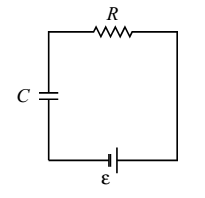
\includegraphics[width=0.3\textwidth]{images/Circuito_RC.png}
    \caption{Representación de un circuito RC de primer orden.}
    \label{fig::circuito_rc_representación}
\end{figure}

Partimos entonces de un condensador de capacidad $C$ completamente descargado conectado en serie a una resistencia de valor $R$. En el instante de tiempo $t=0s$, aplicamos una diferencia de potencial $\varepsilon$ , cuyo valor coincide con el voltaje característico de la fuente utilizada (figura \ref{fig::circuito_rc_representación}).\\


En ese mismo instante, la carga del condensador es nula, así que utilizando la definición de capacidad del condensador (\ref{def::capacidad_conductor}) llegamos a la conclusión de que el potencial en él también es cero. Por otro lado, tenemos que la energía potencial entre los bornes de la resistencia ha de ser máxima, y por consiguiente la intensidad de corriente que circula a través de ella también ha de serlo. Esto se debe principalmente a que debe de cumplirse el principio de conservación de la energía; que si hablamos en términos de potencial eléctrico, lo podemos traducir en que la energía suministrada por la fuente debe de ser en todo momento igual a la consumida por los componentes pasivos del circuito: el condensador y la resistencia.


\begin{figure}[!h]
    \centering
    \subfloat[$t = 0s$]{
        \label{fig::circuito_rc2}
        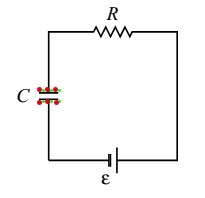
\includegraphics[width=0.33\textwidth]{images/Circuito_RC_2.png}
    }
    \subfloat[Proceso de carga.]{
        \label{fig::circuito_rc3}
        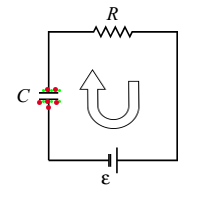
\includegraphics[width=0.33\textwidth]{images/Circuito_RC_3.png}
    }
    \subfloat[Carga completa]{
        \label{fig::circuito_rc4}
        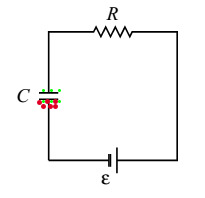
\includegraphics[width=0.33\textwidth]{images/Circuito_RC_4.png}
    }
    \caption{Fases del estado de carga de un condensador. Los puntos rojos hacen referencia a los electrones en movimiento, los puntos verdes a las cargas positivas. La flecha indica el sentido del movimiento de los electrones.}
    \label{fig::carga_condensador}
\end{figure}


Este principio, debe de mantenerse durante todo el proceso de carga hasta que la diferencia de potencial en el condensador sea máxima, y por tanto lo sea la carga almacenada en él. Como debe de volver a cumplirse el principio de conservación energético, ahora la energía potencial entre los bornes de la resistencia es cero, y utilizando de nuevo la Ley de Ohm, tenemos que la intensidad de corriente ha de ser nula. Matemáticamente, podemos expresar este balance utilizando la siguiente ecuación diferencial:
\begin{equation}
    \varepsilon = V_C(t) + V_R(t) = \frac{q(t)}{C} + R\frac{d q(t)}{d t}
    \label{eqq::balance_energetico_rc_1}
\end{equation}

, dónde $\varepsilon$ es la energía suministrada por la fuente por cada unidad de carga que la atraviesa, $V_C(t)$ es la \textit{ddp} en el condensador y $V_R(t)$ la diferencia de potencial en la resistencia. Si la resolvemos, podemos obtener las expresiones recogidas en la tabla \ref{tab::ecuaciones_carga_rc}.\\


\begin{table}[!ht]
    \begin{center}
        \begin{tabular}{|| c | c | c ||}
            \hline
            \textbf{Concepto} & \textbf{Expresión} &  \textbf{Resolución}\\ \hline
            Carga del condensador & $q(t) = C\varepsilon \left( 1 - e^{\frac{-t}{RC}} \right)$ & \ref{part::carga_condensador_1} \\
            Intensidad de corriente & $I(t) = \frac{\varepsilon}{R}e^{\frac{-t}{RC}}$ & \ref{part::carga_condensador_2} \\
            Diferencia de potencial resistencia & $V_R(t) = \varepsilon \cdot e^{\frac{-t}{RC}}$ & \ref{part::carga_condensador_3} \\ 
            Diferencia de potencial condensador & $V_C(t) = \varepsilon \left(1- e^{\frac{-t}{RC}}\right)$ & \ref{part::carga_condensador_4} \\ 
            Energía del condensador & $E(t) = \frac{1}{2}CV_C(t)^2 $ & \ref{part::energia_condensador}
            \\
            \hline
            \end{tabular}
            \caption{Modelado del estado de carga del condensador.}
            \label{tab::ecuaciones_carga_rc}
    \end{center}
\end{table}

Sin embargo, si tenemos un circuito sin fuente de fuerza electromotriz y partimos de un condensador previamente cargado con una carga $q_{max}$ y de capacidad $C$, conectado a una resistencia $R$ en serie, el escenario en el que nos encontramos es diferente.\\ 

En el mismo instante en el que cerramos el circuito ($t=0s$) los electrones libres de la armadura cargada negativamente provocan una corriente eléctrica en el circuito desplazándose hacia la placa de carga positiva. Dicha corriente, ocasiona una disminución del potencial eléctrico en la resistencia y, como debe de cumplirse el principio de conservación de la energía y no se dispone de una fuente de energía, el condensador hace las veces de ésta y el potencial en el mismo se incrementa de forma que el balance energético en el circuito es cero (ambos se anulan entre sí). \\

Como ya se ha comentado, no existe una fuente de energía que aplique un potencial a los componentes del circuito, es por eso que la suma de los potenciales de la resistencia y el condensador debe de ser cero en todo momento. Podemos plantear la ecuación diferencial (\ref{eqq::balance_energetico_rc_2}) para estudiar el comportamiento del circuito en el estado de descarga del condensador.

\begin{figure}[!h]
    \centering
    \subfloat[$t=0$. Carga previa.]{
        \label{fig::circuito_rc5}
        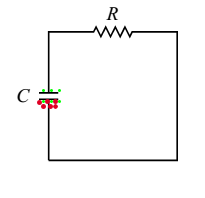
\includegraphics[width=0.33\textwidth]{images/Circuito_RC_5.png}
    }
    \subfloat[Proceso de descarga]{
        \label{fig::circuito_rc6}
        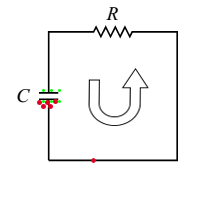
\includegraphics[width=0.33\textwidth]{images/Circuito_RC_6.png}
    }
    \subfloat[Condensador con $q=0$]{
        \label{fig::circuito_rc7}
        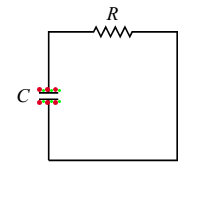
\includegraphics[width=0.33\textwidth]{images/Circuito_RC_7.png}
    }
    \caption{Fases del estado de descarga de un condensador. Los puntos rojos hacen referencia a los electrones en movimiento.}
    \label{fig::descarga_condensador}
\end{figure}
\begin{equation}
    0 = V_C(t) + V_R(t) = \frac{q(t)}{C} + R\frac{d q(t)}{d t}
    \label{eqq::balance_energetico_rc_2}
\end{equation}
\hphantom{1}\\
Si resolvemos la ecuación diferencial planteada (\ref{eqq::balance_energetico_rc_2}) podemos obtener las expresiones que se muestran en la tabla \ref{tab::ecuaciones_descarga_rc} que modelan el comportamiento de las diferentes magnitudes físicas de la descarga de un condensador; suponiendo que la carga inicial del mismo es la máxima permitida.\\



\begin{table}[!ht]
    \begin{center}
        \begin{tabular}{|| c | c | c ||}
            \hline
            \textbf{Concepto} & \textbf{Expresión} &  \textbf{Resolución}\\ \hline
            Carga del condensador & $q(t) = q_{max} e^{-t/{RC}}$ & \ref{part::descarga_condensador_1} \\
            Intensidad de corriente & $I(t) = \frac{-\varepsilon}{R}e^{\frac{-t}{RC}}$ & \ref{part::descarga_condensador_2} \\
            Diferencia de potencial resistencia & $V_R(t) = -\varepsilon \cdot e^{\frac{-t}{RC}}$ & \ref{part::descarga_condensador_3} \\ 
            Diferencia de potencial condensador & $V_C(t) = \varepsilon   e^{\frac{-t}{RC}}$ & \ref{part::descarga_condensador_4} \\ 
            Energía del condensador & $E(t) = \frac{1}{2}CV_C(t)^2 $ & \ref{part::energia_condensador} \\
            \hline
            \end{tabular}
            \caption{Expresiones que modelan la descarga del condensador}
            \label{tab::ecuaciones_descarga_rc}
    \end{center}
\end{table}


\newpage
Si estudiamos las expresiones matemáticas de cada una de las magnitudes físicas del circuito, observamos que todas ellas dependen del tiempo transcurrido $t$; es decir, las magnitudes de un circuito RC de primer orden varían a lo lo largo del tiempo. Además, este tiempo se ve afectado por un valor constante que viene dado por el producto de la capacidad del condensador y del valor óhmico de la resistencia. Definimos a este valor como la \textit{constante de tiempo RC} (\ref{eqq::constante_tiempo_rc}). 

Esa constante, indica el tiempo que ha de transcurrir para que el condensador alcance el $63.2\%$ de su carga máxima; o dicho de otra manera, es el tiempo que tarda el condensador en cargarse completamente si la corriente fuese siempre la inicial. Cuanto menor sea este valor, más rápida es la carga o la descarga del condensador.
\begin{equation}
    \tau_{RC} = R \cdot C
    \label{eqq::constante_tiempo_rc}
\end{equation}

Para comprobar que efectivamente el comportamiento de cada una de las magnitudes es el esperado, vamos a analizar los resultados de un circuito de ejemplo, tomando una fuente con un voltaje de $\varepsilon = 6V$, una resistencia $R=1000\Omega$ y un condensador de capacidad $C=10 \mu F$. Para ello, vamos a utilizar un \textit{script} de \textit{python} que, dado estos datos, nos devuelve las gráficas de ambos estados del circuito.

\begin{figure}[h!]
    \centering
    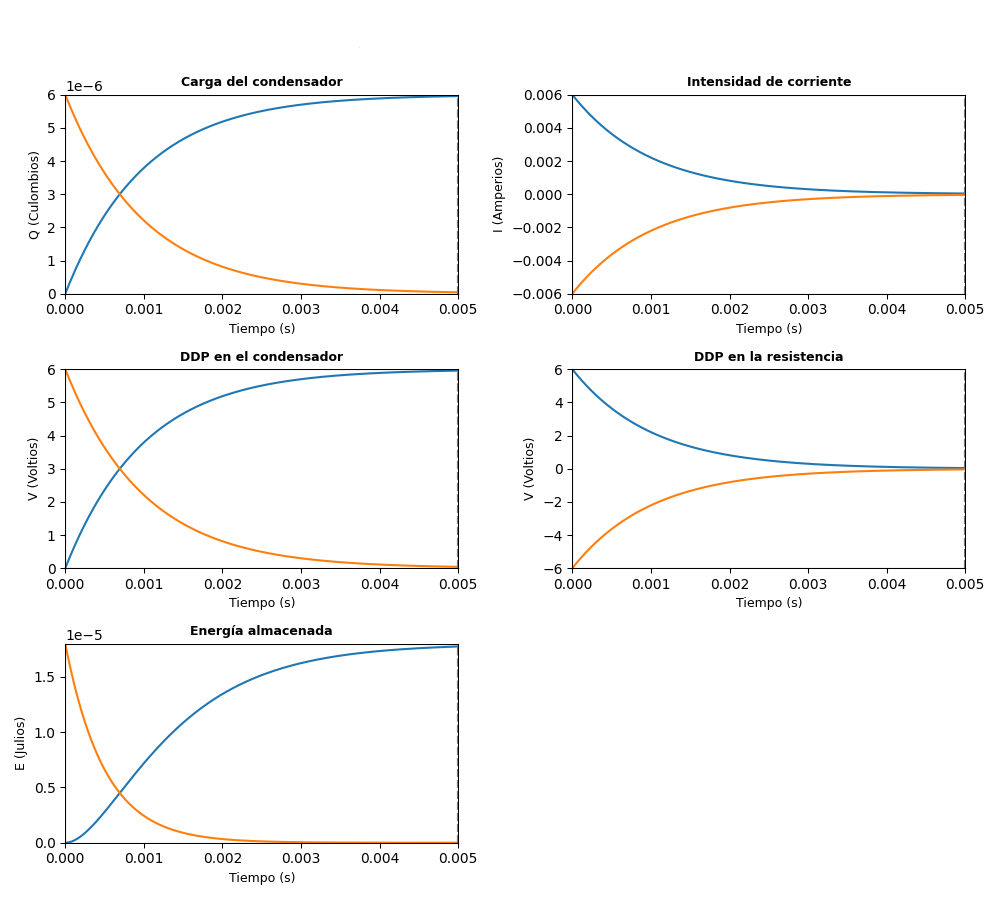
\includegraphics[width=0.9\textwidth]{images/resultados_ejemplo_circuitoRC.png}
    \caption{Simulación de carga(azul) y descarga(naranja) de un condensador, para $\varepsilon=6V$, $R=1000 \Omega$ y $C=10 \mu F$.}
    \label{fig::sim_ejemplo_rc}
\end{figure}

\newpage
Analizamos entonces los resultados obtenidos (figura \ref{fig::sim_ejemplo_rc}). Cuando el circuito se encuentra dispuesto para la carga del condensador, podemos observar que a medida que transcurre el tiempo, la carga de este dispositivo aumenta y, por lo tanto lo hacen la diferencia de potencial y la energía almacenada en el mismo. Puesto que el número de electrones que pueden desplazarse de una placa a la otra del condensador será cada vez menor, la intensidad de corriente irá disminuyendo hasta ser prácticamente cero. De la misma forma, el potencial en la resistencia también disminuye.\\ 

En el proceso de descarga, el movimiento de los electrones es en sentido contrario a la carga, y por lo tanto también lo sería la intensidad de corriente. El condensador actúa como una pila, por lo que el desplazamiento de los electrones de la armadura cargada negativamente hacia la otra hace que la carga del condensador disminuya, igual que la diferencia de potencial y la energía almacenada, hasta ser cero.\\

Además, como la constante de tiempo es muy pequeña, el tiempo empleado en la carga y descarga es de apenas 0.005 segundos. Si utilizamos una resistencia mayor, por ejemplo de $1M \Omega$, el tiempo en completarse la carga o la descarga del condensador asciende hasta los 5 segundos (figura \ref{fig::sim_ejemplo_rc2}).


\begin{figure}[h!]
    \centering
    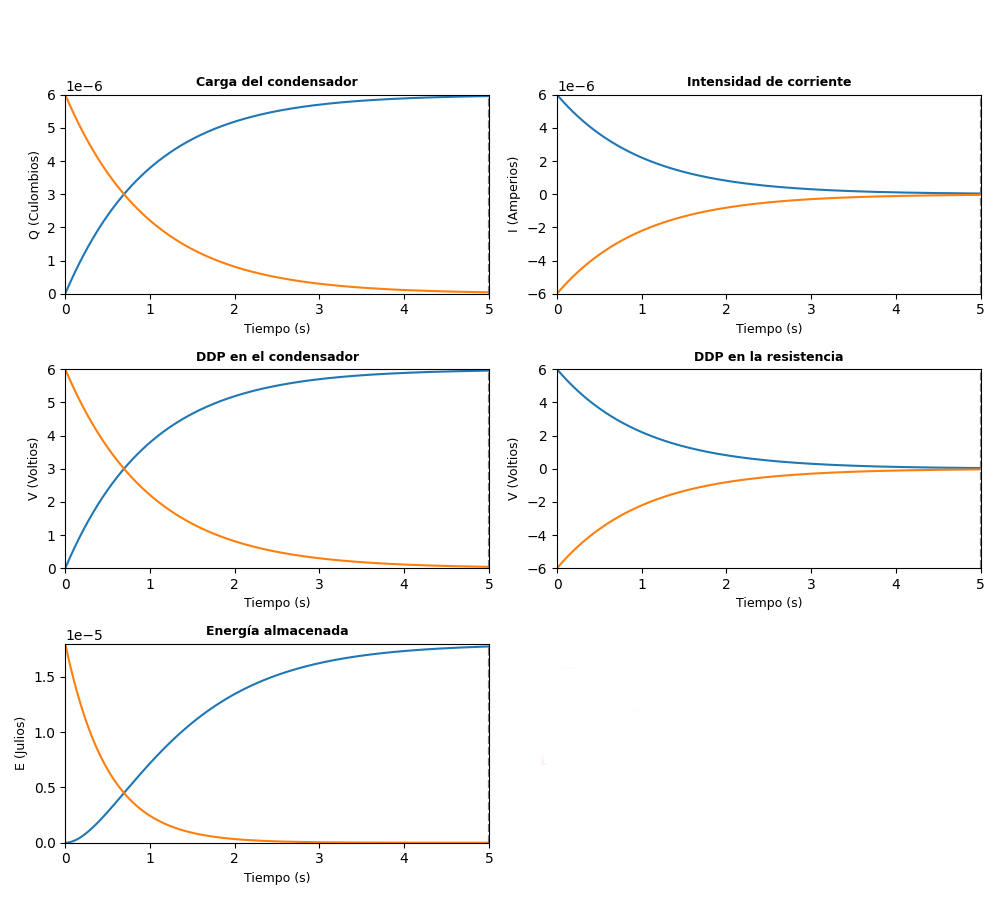
\includegraphics[width=0.9\textwidth]{images/resultados_ejemplo_circuitoRC2.png}
    \caption{Simulación de carga (azul) y descarga(naranja) de un condensador, para $\varepsilon=6V$, $R=1M \Omega$ y $C=10 \mu F$.}
    \label{fig::sim_ejemplo_rc2}
\end{figure}

\newpage
\subsection{El inductor y el circuito RL}
Tal y como se comentó durante la introducción de este capitulo, podemos hacer uso de los circuitos RL para incrementar la intensidad de corriente y así, conseguir por ejemplo, aumentar la tensión y crear un arco voltaico con energía suficiente para quemar combustible en un motor de gasolina. Para ello, utilizaremos la bobina, un dispositivo compuesto por un hilo conductor enrollado alrededor de un núcleo, normalmente de aire o de algún material ferruginoso (como el hierro o la ferrita).\\ 

Supongamos entonces que tenemos una bobina y provocamos una intensidad de corriente eléctrica utilizando cualquier fuente de energía, como una pila. Esta variación de corriente (que inicialmente supondremos como nula) produce en el espacio de la bobina una perturbación conocida como \textit{campo magnético}, y que por sus propiedades, afecta a todos los objetos que presentan una naturaleza similar; que en este caso, serían las cargas en movimiento de la corriente eléctrica. \\

\begin{figure}[!h]
    \centering
    \subfloat[Bobina toroidal con núcleo férrico]{
        \label{fig::bobina_toroidal}
        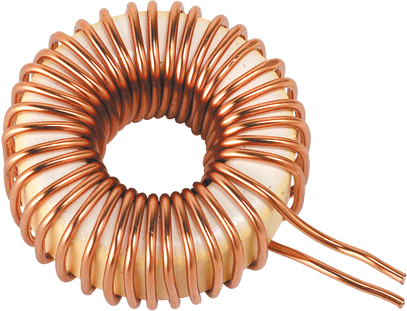
\includegraphics[width=0.33\textwidth]{images/bobina_toroidal.png}
    }
    \subfloat[Bobina espiral con núcleo de aire]{
        \label{fig::bobina_espiral}
        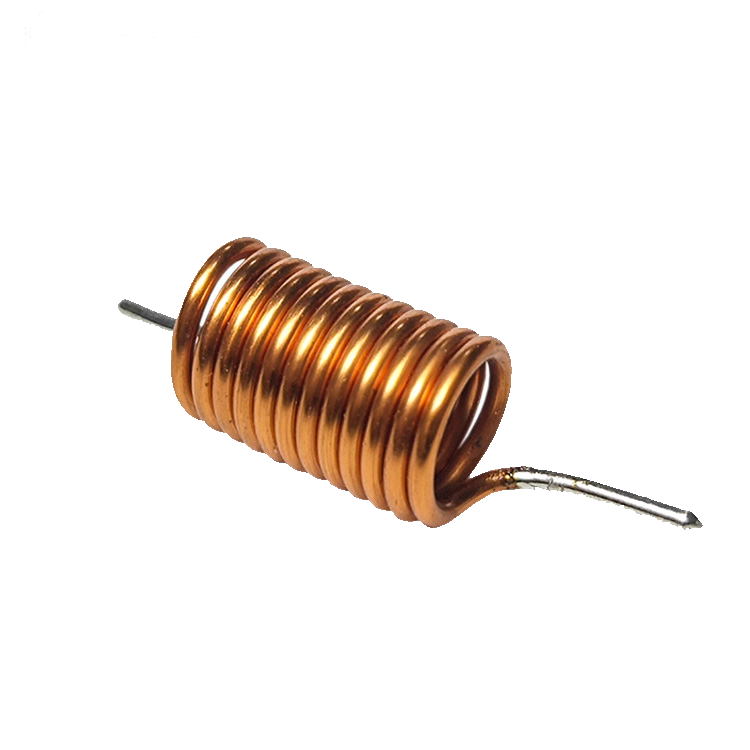
\includegraphics[width=0.33\textwidth]{images/bobina_espiral.png}
    }
    \caption{Tipos de bobinas}
    \label{fig::tipos_bobinas}
\end{figure}

Puesto que esa intensidad de corriente a cambiado, el campo magnético creado por este movimiento de cargas también se ve afectado y como consecuencia, volverá a alterar el valor de la intensidad. A esto se le conoce como el \textit{fenómeno de autoinducción}, produciendo en la bobina una F.E.M autoinducida cuya valor es directamente proporcional a la variación de flujo magnético; es decir, a la cantidad de campo magnético que atraviesa la superficie de la bobina. A esta magnitud que relaciona intensidad de corriente y flujo magnético recibe el nombre de \textit{coeficiente de autoinducción}, cuyo valor depende exclusivamente de la geometría y el medio en el que se encuentre la bobina, siendo su unidad de medida el \textit{henrio} ($H$). Pero al igual que ocurría con el caso de los condensadores, para simplificar los cálculos, no se va a tener en cuenta ni la geometría ni el medio donde se encuentre, sino que directamente haremos uso del coeficiente de autoinducción asociado. \\ 

\begin{figure}[!h]
    \centering
    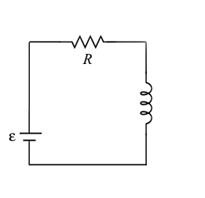
\includegraphics[width=0.3\textwidth]{images/Circuito_RL.png}
    \caption{Representación de un circuito RL de primer orden.}
    \label{fig::circuito_rL_representación}
\end{figure}


Ya sabiendo qué es una bobina, un circuito RL es un conjunto de resistencias eléctricas y bobinas conectadas a una fuente de alimentación. El principal objetivo es comprender la evolución de las diferentes magnitudes físicas que afectan al circuito al inducir corriente eléctrica con estos dispositivos; así que en lugar de analizar un circuito complejo, el análisis y la simulación del mismo se realizará sobre un circuito RL de primer orden. Esto es, un circuito formado por una resistencia y una bobina conectadas en serie. \\

Partimos entonces de un circuito RL de primer orden, donde inicialmente supondremos que la intensidad de corriente que circula por él es nula. En el momento en el que aplicamos una diferencia de potencial al circuito utilizando una fuente de alimentación con un voltaje característico $\varepsilon$, se produce una emisión de cargas negativas desde el terminal con carga negativa de la pila. El movimiento de estas cargas provocan un campo magnético en la bobina cuando esta es atravesada por la corriente eléctrica generada. Además, en estado transitorio, esta corriente aumenta y por tanto el campo y el flujo magnético en la misma, originando un fenómeno de autoinducción según el cual, la bobina se opone a que la corriente cambie, relantizando en el tiempo el incremento de ésta. 

\begin{figure}[!h]
    \centering
    \subfloat[Instante inicial. Intensidad nula.]{
        \label{fig::circuito_rl_1 }
        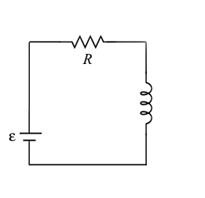
\includegraphics[width=0.33\textwidth]{images/Circuito_RL.png}
    }
    \subfloat[Autoinducción de corriente (carga)]{
        \label{fig::circuito_rl_2}
        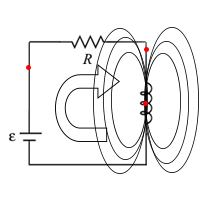
\includegraphics[width=0.33\textwidth]{images/Circuito_RL_2.png}
    }
    \caption{Almacenamiento de energía magnética en una bobina. La flecha indica la dirección de la intensidad de corriente, por lo que el movimiento de los electrones es en sentido contrario.}
    \label{fig::carga_bobina}
\end{figure}

Por supuesto, el \textit{principio de conservación de la energía} debe de cumplirse. Si bien el potencial en los bornes de la bobina disminuye a medida que se incrementa la intensidad de corriente, la diferencia de potencial en la resistencia aumenta. Cuando esta ddp en la resistencia se iguale al valor de la fuente $\varepsilon$, la intensidad del circuito será máxima y por lo tanto, la energía almacenada en el inductor en forma de campo magnético también lo es. Obtenemos entonces las expresiones que modelan el circuito RL realizando un balance energético en términos de potencial del circuito.
\begin{equation}
    \label{eqq::carga_bobina}
    \varepsilon = V_L(t) + V_R(t) = L \frac{d I(t)}{d t} + R I(t)
\end{equation}

, dónde $V_L(t)$ es la diferencia de potencial en el inductor y $V_R(t)$ en la resistencia. De esta ecuación, podemos deducir las expresiones que se muestran en la tabla \ref{tab::ecuaciones_carga_rl}.

\begin{table}[!ht]
        \begin{center}
            \begin{tabular}{|| c | c | c ||}
                \hline
                \textbf{Concepto} & \textbf{Expresión} &  \textbf{Resolución}\\ \hline
                Intensidad de corriente & $I(t) = \frac{\varepsilon}{R} \left( 1 - e^{\frac{-Rt}{L}}\right)$ & \ref{part::carga_inductor_1}\\
                Diferencia de potencial resistencia & $V_R(t) = \varepsilon \left( 1 - e^{\frac{-Rt}{L}}\right)$ & \ref{part::carga_inductor_2} \\ 
                Diferencia de potencial inductor & $V_L(t) = \varepsilon   e^{\frac{-Rt}{L}}$ & \ref{part::carga_inductor_3} \\ 
                Energía del inductor & $E(t) = \frac{1}{2}LI(t)^2 $ & \ref{part::energía_inductor} \\
                Flujo magnético & $\phi (t) = L \cdot I(t)$ & \ref{part::flujo_magnetico_inductor} \\
                \hline
                \end{tabular}
                \caption{Expresiones que modelan la carga de la bobina}
                \label{tab::ecuaciones_carga_rl}
        \end{center}
    \end{table}

\hphantom{1}\\    
Por otro lado, una vez que la corriente que circula por el circuito alcanza su valor máximo y es constante, cesa la autoinducción y la bobina almacena energía magnética (figura \ref{fig::circuito_rl_2}). El proceso de disipación de la energía almacenada en el campo magnético de la bobina comienza cuando quitamos la fuente de fuerza electromotriz y deja de suministrar energía, es decir, cuando $\varepsilon = 0$ (figura \ref{fig::circuito_rl_3}). \\
    

 \begin{figure}[!h]
    \centering
    \subfloat[Instante inicial. Intensidad máxima.]{
        \label{fig::circuito_rl_3}
        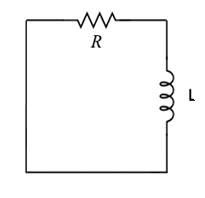
\includegraphics[width=0.33\textwidth]{images/Circuito_RL_4.png}
    }
    \subfloat[Intensidad nula.]{
        \label{fig::circuito_rl_4}
        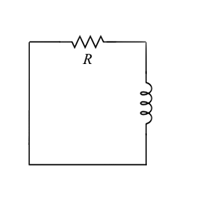
\includegraphics[width=0.33\textwidth]{images/Circuito_RL_5.png}
    }
    \caption{Disipación de energía magnética en una bobina. La flecha indica la dirección de la intensidad de corriente.}
    \label{fig::carga_bobina}
\end{figure}

Toda la energía cinética de las cargas en movimiento se disipan en forma de calor en la resistencia eléctrica del circuito, disminuyendo así la intensidad de corriente hasta ser cero. Puesto que la intensidad ha sufrido una variación respecto a su valor inicial, el campo magnético sufre variaciones (de nuevo por el fenómeno de autoinducción). Además, conforme la intensidad disminuye también lo hacen las tensiones de la resistencia y el inductor, y con ellos la energía almacenada y el flujo magnético de la bobina. Realizando un nuevo balance energético del circuito, obtenemos la siguiente ecuación a resolver, 
\begin{equation}
    \label{eqq::descarga_bobina}
    0 = V_L(t) + V_R(t) = L \frac{d I(t)}{d t} + R I(t)
\end{equation}

, a partir de la cuál podemos deducir las expresiones que modelan el comportamiento de cada una de las magnitudes físicas que afectan al circuito durante la descarga de la bobina, tal y como se muestran en la tabla \ref{tab::ecuaciones_descarga_rl}.\\

\begin{table}[!ht]
        \begin{center}
            \begin{tabular}{|| c | c | c ||}
                \hline
                \textbf{Concepto} & \textbf{Expresión} &  \textbf{Resolución}\\ \hline
                Intensidad de corriente & $I(t) = \frac{\varepsilon}{R}  e^{\frac{-Rt}{L}}$ & \ref{part::descarga_inductor1}\\
                Diferencia de potencial resistencia & $V_R(t) = \varepsilon  e^{\frac{-Rt}{L}}$ & \ref{part::descarga_inductor_2} \\ 
                Diferencia de potencial inductor & $V_L(t) = - \varepsilon   e^{\frac{-Rt}{L}}$ & \ref{part::descarga_inductor_3} \\ 
                Energía del inductor & $E(t) = \frac{1}{2}LI(t)^2 $ & \ref{part::energía_inductor} \\
                Flujo magnético & $\phi (t) = L \cdot I(t)$ & \ref{part::flujo_magnetico_inductor} \\
                \hline
                \end{tabular}
                \caption{Expresiones que modelan la descarga de la bobina}
                \label{tab::ecuaciones_descarga_rl}
        \end{center}
    \end{table}

Como podemos observar todas las magnitudes físicas dependen del tiempo ($t$), el cuál se encuentra afectado por el coeficiente de autoinducción de la bobina y del valor óhmico de la resistencia. A este valor, lo llamaremos \textit{constante de tiempo RL}. Este, indica la velocidad de reacción del circuito y, cuanto más pequeño sea este valor, antes se alcanzará el valor máximo de corriente eléctrica. Denotamos a esta constante con el símbolo $\tau_{RL}$

\begin{equation}
    \label{eqq::constante_tiempo_rl}
    \tau_{RL} = \frac{L}{R}
\end{equation}

Comprobamos entonces que el comportamiento de cada una de las magnitudes físicas es el adecuado, analizando un circuito RL de primer orden con una fuente de alimentación de $\varepsilon = 6V$, una resistencia eléctrica $R=1\Omega$ y una bobina con un coeficiente de autoinducción $L=10mH$. \\



\begin{figure}[!h]
    \centering
    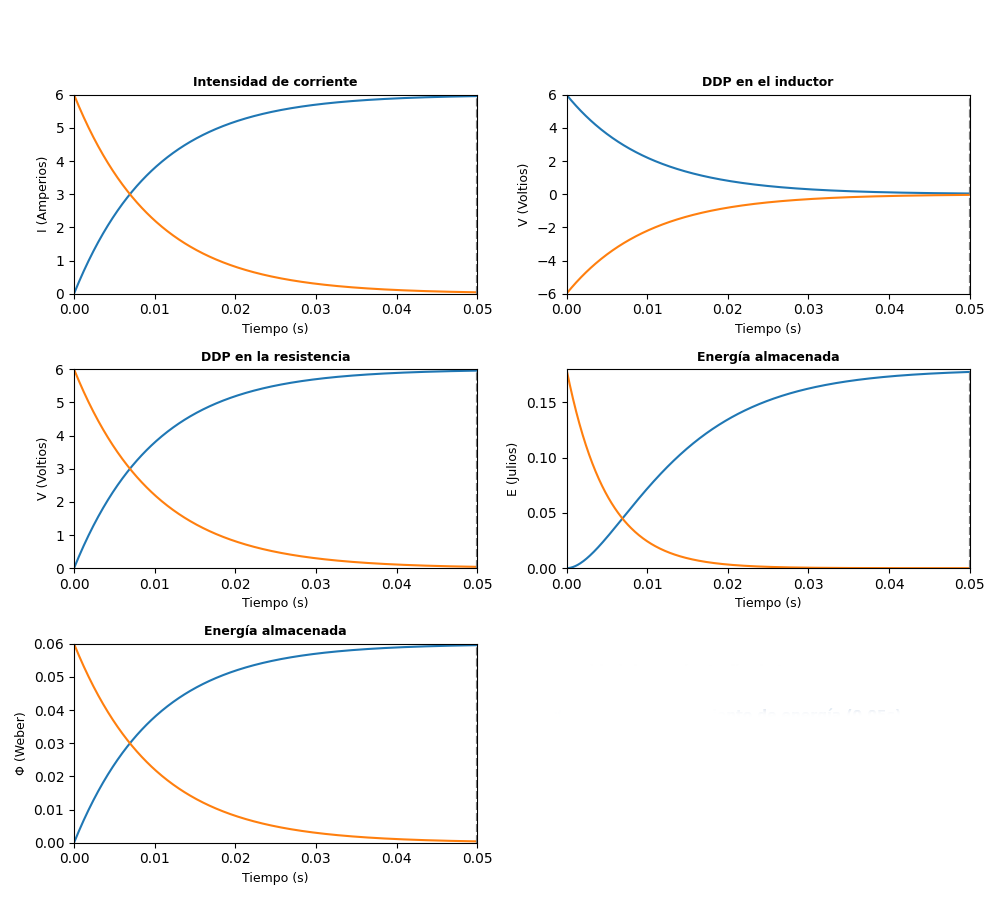
\includegraphics[width=\textwidth]{images/resultados_ejemplo_circuitoRL.png}
    \caption{Simulación almacenamiento de energía (azul) y disipación de energía (naranja) magnética de una bobina, para $\varepsilon=6V$, $R=1 \Omega$ y $L=10 mH$.}
    \label{fig::sim_ejemplo_rl}
\end{figure}


Analizamos entonces los resultados que hemos obtenido en la figura \ref{fig::sim_ejemplo_rl}. Cuando el circuito se encuentra en disposición para almacenar energía en la bobina, debido al fenómeno de autoinducción, tanto la intensidad de corriente como la cantidad de campo magnético aumentan; y por lo tanto, lo hacen la energía magnética que se almacena en este dispositivo y la diferencia de potencial de la resistencia. Esta última, como se puede ver en los resultados, aumenta hasta tener un valor igual al de la fuente de alimentación. Como además debe de cumplirse el principio de conservación energético, la diferencia de potencial en la bobina cae hasta ser cero.\\ 

Por otro lado cuando partimos de una intensidad de corriente máxima en el circuito y eliminamos la fuente de alimentación, la propia bobina actúa como un generador. Así que podremos observar como se sufre una caída en la intensidad de corriente, por lo que tanto la energía magnética almacenada como la energía potencial en la resistencia y el inductor, disminuirán hasta que la corriente que circula por el circuito sea completamente cero. En otras palabras, la energía magnética que quedará almacenada en la bobina será nula.



\end{document}